% !TEX encoding = UTF-8 Unicode
\documentclass[12pt]{article}
\usepackage{geometry}                % See geometry.pdf to learn the layout options. There are lots.
\geometry{a4paper}                   % ... or a4paper or a5paper or ... 
%\geometry{landscape}                % Activate for for rotated page geometry
%\usepackage[parfill]{parskip}    % Activate to begin paragraphs with an empty line rather than an indent
\usepackage{graphicx}
\usepackage{amssymb}
\usepackage{epstopdf}
\usepackage[T1]{fontenc}
\usepackage[utf8]{inputenc}
\usepackage{hyperref}

\renewcommand{\labelitemi}{$-$}

\DeclareGraphicsRule{.tif}{png}{.png}{`convert #1 `dirname #1`/`basename #1 .tif`.png}

% here insert the full path to your BibTeX file
\newcommand{\myreferences}{/Users/matteo/Documents/library.bib}

\title{L'analisi dei movimenti oculari come strumento di indagine dei processi cognitivi}
\author{
        Matteo Lisi \footnote{\scriptsize{Questo capitolo è stato scritto mentre l'autore lavorava presso Laboratoire Psychologie de la Perception, Université Paris Descartes, Parigi. Una versione di questo capitolo è in corso di pubblicazione nel volume \href{https://www.mulino.it/isbn/9788815272119}{\textit{Il cervello al lavoro. Nuove prospettive in neuropsicologia} curato da Patrizia Bisiacchi e Antonino Vallesi (2017, editore il Mulino, ISBN 978-88-15-27211-9)}.}} \\
        \small{Department of Optometry \& Visual Science}\\
        \small{City, University of London}
}
\date{}

\begin{document}
\sloppy
\maketitle

\begin{abstract}
Lo studio dei movimenti oculari \`e un'importante fonte di informazioni sia per la psicologia e neuropsicologia clinica che per quella sperimentale. Nella prima parte di questo capitolo verranno descritte le differenti tipologie di movimenti oculari e le loro funzioni. Nella seconda parte del capitolo verrà discussa la relazione tra movimenti oculari e percezione visiva, e verranno presentati alcuni casi di studio in cui l'analisi dei movimenti oculari ha permesso di ottenere informazioni importanti riguardo a processi cognitivi come l'attenzione e la cognizione numerica. Anche se il capitolo sarà perlopiù dedicato ai movimenti di rotazione dell'occhio nell'orbita, verranno trattati brevemente anche i movimenti di dilatazione e restringimento della pupilla. Il capitolo si concluderà con una breve descrizione delle tecniche e metodologie utilizzate per la registrazione dei movimenti oculari.
\end{abstract}

\section{Tassonomia e funzione dei movimenti oculari}
I movimenti oculari si trovano all'intersezione tra le funzioni motorie e quelle percettive del cervello. Da un lato si tratta di un'azione motoria: l'atto di muovere gli occhi inizia con l'attivazione di una popolazione di neuroni, e termina con una contrazione o rilassamento dei muscoli oculari nell'orbita. I movimenti oculari, tuttavia, svolgono una funzione ben precisa: permettere la percezione visiva, cio\`e l'elaborazione di informazioni provenienti dal mondo esterno attraverso il senso della visione. 

La visione inizia quando la luce penetra nell'occhio interno e raggiunge la retina, modulando l'attivit\`a dei fotorecettori. \`E ben noto che l'acutezza visiva (definibile grossolanamente come la chiarezza della visione, cio\`e la capacità del sistema visivo di risolvere e percepire dettagli fini nella scena visiva) non \`e uniforme nel campo visivo: \`e massima nella regione centrale, in corrispondenza della \textit{fovea}, cioè la parte della retina dove vi \`e la massima densità di fotorecettori, e decresce in maniera esponenziale con la distanza dal centro (cf. fig.\ref{fig1}). Persino all'interno della fovea l'acutezza visiva non \`e uniforme e raggiunge l'apice in una regione molto limitata (chiamata \textit{foveola}), circa 0.3 mm di diametro, che corrispondono a circa 1 grado di angolo visivo\footnote{I gradi di angolo visivo ($^{\circ}$) sono le unit\`a di misura in cui si misurano sia le rotazioni dell'occhio, che la dimensione e posizione di oggetti nel campo visivo. Per esempio, se uno stimolo visivo è posizionato a 10$^{\circ}$ di distanza in una certa direzione rispetto al centro del campo visivo, per centrarlo sulla fovea l'occhio deve compiere una rotazione nell'orbita di 10$^{\circ}$ nella stessa direzione. L'angolo visivo $\alpha$ (in gradi) sottinteso da un oggetto di lunghezza $l$ posizionato alla distanza $d$ dall'occhio può essere calcolato con la seguente formula $\alpha = 2 \arctan(\frac{l}{2d}) \frac{180}{\pi}$. Approssimativamente, un oggetto lungo 1 cm e posizionato a 57 cm dall'occhio sottende 1$^{\circ}$.}. A dispetto della sua piccola dimensione, la fovea riveste un'enorme importanza nell'elaborazione dell'informazione visiva: si stima che circa il 50\% della corteccia visiva sia dedicato all'elaborazione dell'informazione proveniente dalla fovea, nonostante questa rappresenti solo l'1\% della retina. 

\begin{figure}
\centering
\includegraphics[width=80mm]{fig1.pdf}
\caption{Il grafico mostra come l'acutezza visiva diminuisca rapidamente quando ci si allontana dalla fovea. rappresentata in funzione della distanza dalla fovea sulla retina. Il \textit{punto cieco}, rappresentato in figura, è il punto in cui i fasci nervosi provenienti dalle varie parti della retina si riuniscono per formare il nervo ottico; siccome il punto cieco non contiene fotorecettori, questa parte della retina non fornisce alcuna informazione visiva.}
\label{fig1}
\end{figure}

Da un punto di vista funzionale quindi i movimenti oculari permettono di orientare lo sguardo (o più precisamente l'asse visivo, cioè la linea immaginaria che connette un oggetto osservato al centro della fovea), in modo che la proiezione sulla retina dell'oggetto di interesse si trovi in prossimità della fovea (dove l'acutezza visiva è massima). Questa strategia (orientare la fovea verso oggetti di interesse) è una soluzione evolutiva che permette al nostro sistema visivo di analizzare velocemente e in dettaglio gli elementi salienti dell'ambiente circostante. Il vantaggio di questa soluzione è la parsimonia: se in tutto il campo visivo avessimo lo stesso livello di acutezza visiva della fovea, la quantità di informazione visiva in ingresso sarebbe tale che per elaborarla avremmo bisogno di una corteccia visiva decine (se non centinaia) di volte più grande! Un'altra importante funzione dei movimenti oculari è di stabilizzare lo sguardo nel caso l'oggetto osservato, oppure l'osservatore (o entrambi) siano in movimento: infatti per mantenere una accettabile qualità della visione è necessario che la velocità dello scivolamento retinico (lo slittamento dell'immagine proiettata sulla retina) sia inferiore a 2-3$^{\circ}$/sec (gradi di angolo visivo al secondo). 

Questi due obiettivi funzionali dei movimenti oculari (orientare e stabilizzare lo sguardo) sono raggiunti attraverso due grandi classi di movimenti distinti: i movimenti rapidi, anche detti movimenti saccadici o saccadi, e i movimenti lenti \cite{Steinman1990}. Le saccadi sono movimenti estremamente rapidi che consentono di spostare lo sguardo da un punto ad un altro del campo visivo. Ad esempio, le saccadi sono i movimenti con i quali avete spostato lo sguardo da una parola all'altra durante la lettura di questo testo. Un esempio di movimento lento è invece fornito dai movimenti di inseguimento, che sono utilizzati per mantenere la fovea orientata verso un oggetto in movimento, come un giocatore che corre o una palla appena calciata durante una partita di pallone. I movimenti lenti sono caratterizzati da un profilo di velocità molto più variabile delle saccadi che dipende in larga parte dalle caratteristiche della stimolazione visiva: per l'esecuzione di un movimento di inseguimento è necessario che qualcosa si muova nel campo visivo, e la velocità di spostamento dello sguardo riflette la velocità dello stimolo. 

I movimenti oculari sono suddivisi  anche in movimenti oculari coniugati, in cui i due occhi si muovono della stessa direzione, e movimenti oculari disgiunti, in cui i due occhi si muovono in direzioni diverse. Un esempio di movimenti disgiunti sono i movimenti di vergenza, che consistono nel convergere o divergere gli occhi in modo da garantire che quando muoviamo lo sguardo da un oggetto lontano verso uno vicino (o viceversa) le proiezioni dell'oggetto di interesse giacciano sulla fovea in entrambe le retine del nostro occhio destro e sinistro. I movimenti di vergenza sono accompagnati dal processo di accomodazione, cioè la regolazione della curvatura del cristallino, l'organo trasparente situato all'interno del bulbo oculare che assieme alla cornea agisce come lente, permettendo la messa a fuoco dei raggi luminosi sulla retina.

I movimenti oculari possono poi essere suddivisi ulteriormente in molteplici sottosistemi, e in letteratura sono stati proposti molteplici schemi di classificazione dei movimenti oculari. In tabella \ref{tab1} è riassunta una delle classificazioni più comunemente utilizzate, dovuta a Robinson \cite{Robinson1968}, che distingue 5 principali tipologie di movimenti oculari. È importante sottolineare che ogni classificazione dipende principalmente dai criteri adottati e che è difficile fare classificazioni "rigide": normalmente le diverse funzioni dell'occhio vengono assolte grazie alla cooperazione di diverse tipologie di movimenti oculari. Per una descrizione più dettagliata delle varie tipologie di movimenti oculari, ivi inclusi quelli di tipo riflesso, si rimanda il lettore a testi specializzati come l'ottimo manuale di Leigh e Zee \cite{Leigh2015}. In questo capitolo ci limiteremo ad approfondire alcuni movimenti oculari volontari, le saccadi e i movimenti di inseguimento lento, che sono forse più interessanti per l'indagine dei processi cognitivi.

\begin{table}
\centering
\caption{Classificazione dei movimenti oculari.} \label{tab1}
\begin{tabular}{p{5.3cm}p{8cm}}
  \hline
\textbf{Tipologia di movimenti oculari}  & \textbf{Funzione}\\ 
  \hline  \hline
 Riflesso vestibolo-oculare & Stabilizzare l'immagine della retina durante movimenti della testa \\  \hline
 Riflesso optocinetico & Stabilizzare l'immagine sulla retina durante slittamento retinico del campo visivo (ad esempio quando da dentro un treno in movimento guardiamo il paesaggio scorrere fuori dal finestrino  \\  \hline
  Saccadi & Spostare lo sguardo in modo da centrare oggetti di interesse sulla fovea  \\  \hline
  Inseguimento lento & Muovere gli occhi per seguire un oggetto in movimento, in modo da mantenerlo centrato sulla fovea  \\  \hline
  Vergenza & Muovere gli occhi in direzioni opposte in modo che le proiezioni di un oggetto siano centrati sulle fovee di entrambi gli occhi simultaneamente  \\  \hline
   \hline
\end{tabular}
\end{table}

\subsection{Tassonomia e funzione dei movimenti oculari}
I movimenti oculari sono determinati dall'azione di 6 muscoli (i cosiddetti muscoli estrinseci dell'occhio), organizzati in 3 coppie ad azione antagonista. Sono costituiti da fibre striate, originano dal foro ottico, nel fondo dell'orbita (dove passa anche il nervo ottico), e terminano inserendosi sulla sclera (lo strato esterno del globo oculare). L'attivazione coordinata di questi muscoli permette al globo oculare di muoversi nell'orbita con 6 gradi di libertà. Tre di questi sono traslazioni, che hanno un ampiezza minima e in questo capitolo verranno trascurate. Le altre 3 sono rotazioni che permettono all'occhio di ruotare intorno a 3 diversi assi, e sono ottenute mediante la contrazione di un muscolo e il rilassamento del suo antagonista. L'attivazione combinata delle 3 coppie di muscoli può far quindi ruotare il globo oculare intorno a 3 assi: un asse verticale, un asse orizzontale, e l'asse visivo (movimenti detti di torsione). Le rotazioni intorno all'asse verticale consentono di eseguire movimenti oculari orizzontali, detti abduzioni quando sono in direzione temporale e adduzioni quando sono in direzione nasale, e sono ottenute mediante la contrazione/rilassamento dei muscoli retti mediali e laterali. Le rotazioni attorno all'asse orizzontale risultano invece in movimenti oculari verticali detti di elevazione e abbassamento. I movimenti oculari verticali, insieme a quelli di torsione, sono ottenuti principalmente grazie al coinvolgimento dei muscoli retti superiore ed inferiore ed obliqui superiore e inferiore. 

I muscoli oculari sono innervati dal III, IV e VI nervo cranico, provenienti dai nuclei oculomotori del tronco encefalico. In particolare il III nervo cranico innerva i muscoli retto superiore, retto mediale, retto inferiore, e obliquo inferiore; il IV nervo cranico innerva il muscolo obliquo superiore, mentre il VI nervo cranico innerva il muscolo retto laterale.

\subsection{Movimenti oculari saccadici}
Le saccadi sono movimenti rapidi e coniugati degli occhi che sono utilizzati per orientare le fovee verso una nuova posizione nella scena visiva. Lo studio delle saccadi risale almeno alla fine del XIX secolo, quando l'oftalmologo francese Louis Émile Javal (1839-1907) osservò che durante la lettura lo sguardo non viene spostato lungo la linea del testo in maniera fluida e continua, ma attraverso una serie di movimenti discreti molto veloci (in francese il termine saccade indica appunto un movimento brusco e rapido), intervallate da momenti di pausa in cui lo sguardo rimane stazionario (fissazioni).

Le saccadi possono essere controllate in maniera volontaria: possiamo sempre decidere quando e dove spostare lo sguardo. Tuttavia nella vita quotidiana vengono perlopiù generate in maniera inconsapevole e automatica: anche se non vi prestiamo attenzione, i nostri occhi non sono mai fermi, e in media effettuiamo 3 saccadi al secondo. Le saccadi possono inoltre essere generate in maniera riflessa/involontaria, in risposta ad uno stimolo improvviso, come per esempio quando qualcosa compare nella periferia del nostro campo visivo attirando la nostra attenzione e il nostro sguardo. Le saccadi non sono limitate a stimoli visivi: ad esempio è stato dimostrato che in completa oscurità la stimolazione tattile di una mano risulta tipicamente in un movimento saccadico diretto verso la mano stimolata \cite{Groh1996}. La latenza di un movimento saccadico in risposta ad uno spostamento dell'oggetto osservato o alla comparsa di un nuovo stimolo periferico si aggira intorno ai 200-250 millisecondi, ed è influenzata da numerosi fattori come luminosità, distanza del bersaglio, presenza di distrattori.

Come abbiamo accennato le saccadi sono dette anche movimenti rapidi: si tratta infatti di uno dei movimenti più veloci prodotti dal corpo umano. Durante una saccade la velocità di rotazione dell'occhio nell'orbita può raggiungere picchi di velocità intorno ai 900$^{\circ}$/sec. Data l'estrema velocità di esecuzione delle saccadi, è naturale che sia molto difficile modificare la loro traiettoria "al volo". Infatti le saccadi sono considerate un tipo di movimento di tipo balistico: una volta iniziato, la sua ampiezza e direzione non possono essere modificate. Inoltre sono caratterizzate da un profilo stereotipato di accelerazione/decelerazione sul quale non abbiamo controllo volontario: iniziano con una rapida accelerazione, che culmina nella prima metà della saccade, seguita da una rapida decelerazione. Vi è un rapporto relativamente stabile tra ampiezza e velocità (e di conseguenza anche durata) di una saccade: la velocità massima aumenta in maniera pressoché lineare con l'ampiezza (vedi figura \ref{fig2}), fino ad ampiezze intorno ai 20$^{\circ}$, che tende ad saturare ed appiattirsi progressivamente per ampiezze superiori ai 20$^{\circ}$. Questa regolarità è definita in letteratura come sequenza principale (main sequence), un termine preso in prestito dall'astronomia (dove indica la relazione tra luminosità e temperatura di una stella), ed è stata utilizzata nell'ambito della ricerca sui movimenti oculari per stabilire se un certo tipo di movimento osservato può essere considerato o meno una saccade (cioè è stato generato dallo stesso sistema di controllo che genera le saccadi) e in ambito clinico per caratterizzare anomalie dei movimenti saccadici. La durata di una saccade quindi dipende dalla sua ampiezza, ma è in generale molto breve: tipicamente intorno ai 50-100 millisecondi per saccadi di ampiezza intorno ai 5-10$^{\circ}$, ma saccadi di ampiezza maggiore possono arrivare fino a 200 millisecondi. 

I movimenti saccadici riorientano l'asse visivo verso elementi di interesse. E' quindi interessante chiedersi con quale accuratezza riescano a centrare i loro bersagli. Bisogna premettere che non tutti i movimenti saccadici sono diretti ad un bersaglio ben definito e di piccole dimensioni (un bersaglio puntiforme): molto spesso le saccadi sono eseguite con il semplice scopo di riposizionare il campo visivo, senza necessariamente essere dirette verso un particolare elemento della scena visiva. 

Per quanto riguarda invece le saccadi dirette verso un bersaglio puntiforme, molti studi hanno mostrato come tendano ad essere non molto accurate: in particolare le saccadi verso bersagli posti a distanze maggiori di circa 5$^{\circ}$ tendono ad essere ipometriche, cioè la loro ampiezza in media tende ad coprire solo il 90\% della distanza del bersaglio \cite{Becker1972}. Sono state proposte diverse teorie per spiegare questo fenomeno: per esempio, poiché la durata di un movimento saccadico tende ad aumentare con la sua ampiezza, è stato suggerito che le saccadi sono programmate in modo da minimizzare il tempo si esecuzione \cite{Harris1995}. Tuttavia è bene ricordare che quando una saccade termina lontano dal suo bersaglio, è tipicamente seguita da una saccade secondaria caratterizzata da piccola ampiezza e latenza molto breve (spesso minore di 100 millisecondi) che corregge l'errore della saccade iniziale \cite{Jacobs1987}. Inoltre in condizioni più ecologiche, dove cioè i bersagli sono stabili (invece di apparire e scomparire all'improvviso come avviene in molti protocolli sperimentali) e il momento di esecuzione del movimento oculare è deciso liberamente dal soggetto, le saccadi tendono ad essere più accurate e a mostrare solo un piccolo errore costante che non aumenta in funzione dell'ampiezza della saccade \cite{Collewijn1988}. Infine, in condizioni ecologiche ogni movimento saccadico è tipicamente accompagnato da un movimento della testa che tende a compensare l'ipometria e ad aumentarne l'accuratezza \cite{Guitton1987}.

\begin{figure}
\centering
\includegraphics[width=140mm]{fig2.pdf}
\caption{Il grafico a sinistra mostra la tipica sequenza principale delle saccadi: una relazione lineare tra ampiezza e il picco di velocità della saccade. Ogni punto rappresenta un movimento saccadico effettuato da un soggetto durante il corso di un esperimento. A destra invece è rappresentato il tracciato oculografico di un singolo movimento saccadico: nel pannello in alto è rappresentata la posizione dello sguardo (calcolata in gradi di angolo visivo rispetto al centro dello uno schermo di computer) in funzione del tempo; notare la tipica forma a gradino, che indica un rapido movimento dello sguardo da una parte all'altra dello schermo. In basso è raffigurata la velocità di spostamento dello sguardo: notare il tipico profilo di rapida accelerazione/decelerazione che caratterizza i movimenti oculari rapidi.}
\label{fig2}
\end{figure}

Come cambia l'accuratezza dei movimenti oculari durante l'invecchiamento? La risposta, per certi versi sorprendente, è che l'accuratezza rimane piuttosto costante \cite{Warabi1984}, mentre altri parametri, come per esempio la durata e la latenza, cambiano significativamente \cite{Munoz1998}. Con l'aumentare dell'età vi sono variazioni fisiologiche, ad esempio nella rigidità dei muscoli oculari, che rendono più difficili i movimenti oculari. Nonostante ciò il nostro sistema oculomotorio è in grado di apprendere, o meglio di adattare gli impulsi che invia ai neuroni oculomotori per contrastare queste variazioni, permettendo di mantenere un livello costante di accuratezza. Questi processi adattivi possono essere dimostrati anche in laboratorio: se chiediamo ad un soggetto di effettuare una saccade per spostare lo sguardo su un bersaglio periferico, ma ogni volta durante l'esecuzione del movimento spostiamo leggermente il bersaglio (ad esempio aumentando  la distanza del 15\%), il sistema oculomotorio si adatterà in breve tempo, e inizierà a rispondere con saccadi sempre più ampie, un fenomeno chiamato adattamento saccadico \cite{McLaughlin1967}. L'adattamento saccadico è una forma di plasticità senso-motoria che, data la facilità con cui può essere elicitata, viene spesso utilizzata come modello sperimentale per lo studio dell'apprendimento senso-motorio.

\subsection{Le fissazioni}
Le fissazioni sono i periodi di pausa - tra un movimento oculare e il successivo - durante i quali avviene la nostra percezione visiva. Le fissazioni hanno una durata molto variabile che dipende da una moltitudine di fattori, legati sia alle caratteristiche dell'immagine osservata che agli obiettivi e stati mentali dell'osservatore. Durante l'esplorazione di una scena visiva si passa da durate minime intorno ai 100 millisecondi, a fissazioni molto più lunghe che possono durare anche più di 2-3 secondi. È importante sottolineare che, dal punto di vista del controllo motorio, le fissazioni non consistono nella semplice assenza di un comando oculomotorio; sono invece il risultato di un sofisticato meccanismo volto a stabilizzare lo sguardo sul bersaglio, in modo da mantenerne l'immagine sulla fovea e permetterne l'analisi da parte del sistema visivo. La stabilizzazione dello sguardo è garantita anche dalla collaborazione del sistema di inseguimento lento, e dei riflessi vestibolo-oculare e optocinetico (vedi Tabella \ref{tab1}).
Sebbene gli occhi appaiano fermi durante le fissazioni, in realtà non sono mai perfettamente immobili ma continuano a muoversi in maniera impercettibile. Questi movimenti microscopici effettuati durante le fissazioni si suddividono in: 
\begin{itemize}
\item \textit{microsaccadi}, cioè movimenti saccadici di piccolissima ampiezza, intorno a 0.1$^{\circ}$;
\item \textit{movimenti di deriva o drift}, movimenti lenti e serpeggianti che si verificano tra una microsaccade e l'altra;
\item \textit{tremore}, una rapida e minuscola oscillazione che si sovrappone ai movimenti di deriva.
\end{itemize}
Questi microscopici movimenti oculari hanno molteplici funzioni. Innanzitutto spostano l'immagine visiva sulla retina, causando continue variazioni nei segnali visivi in ingresso e permettendo di evitare fenomeni di adattamento neurale che potrebbero causare l'evanescenza progressiva delle parti statiche della scena visiva (un fenomeno conosciuto come effetto Troxler, descritto per la prima volta dal filosofo svizzero Ignaz Paul Vital Troxler nei primi anni dell'800). 

In aggiunta studi più recenti hanno dimostrato che questi movimenti microscopici, sempre presenti durante le fissazioni oculari, riformattano l'informazione visiva in ingresso in modo da equalizzare lo spettro di frequenze spaziali che compongono l'immagine, enfatizzando le frequenze spaziali più alte \cite{Rucci2015} e migliorando quindi la sensibilità ai dettagli fini dell'immagine. Infine è stato dimostrato che le microsaccadi possono essere utilizzate anche per posizionare gli oggetti di interesse in corrispondenza della foveola durante compiti che richiedono la percezione di dettagli particolarmente fini, nell'ordine di qualche centesimo di grado di angolo visivo \cite{Ko2010a,Rucci2007}. 

\subsection{I movimenti di inseguimento lento}
I movimenti di inseguimento lento hanno come obiettivo mantenere sulle fovee le immagini di oggetti in movimento. Da un punto di vista motorio sono molto simili al riflesso optocinetico; tuttavia mentre il riflesso optocinetico è generato in maniera riflessa in risposta allo scivolamento retinico dell'intero campo visivo, il movimento di inseguimento è generato in maniera volontaria per mantenere sulla fovea un oggetto che si muove in maniera indipendente rispetto al contesto in cui è posizionato. L'esecuzione di un movimento di inseguimento lento è caratterizzata da una latenza (l'intervallo che intercorre dall'inizio del movimento del bersaglio all'inizio del movimento oculare) di circa 100 millisecondi. 

A dispetto della loro connotazione come movimenti "lento", questi movimenti oculari possono raggiungere velocità piuttosto elevate, fino a circa 100 $^{\circ}$/sec. L'efficienza di questo movimento viene quantificata calcolandone il guadagno, cioè il rapporto tra la velocità di movimento dello sguardo e la velocità del bersaglio. Un valore di guadagno uguale a 1 indicherebbe quindi che gli occhi si muovono alla stessa velocità del bersaglio; tuttavia il guadagno dei movimenti di inseguimento lento è tipicamente inferiore a 1, in particolare per velocità del bersaglio molto elevate. Poiché il guadagno tende ad essere inferiore a 1, per evitare che lo sguardo rimanga indietro rispetto al bersaglio, vengono spesso eseguite saccadi di piccola ampiezza, che servono a ridurre e mantenere a livelli accettabili il distacco tra bersaglio e asse visivo.

Nonostante venga iniziato in maniera volontaria, il movimento di inseguimento lento è interamente determinato dallo stimolo visivo. È infatti impossibile muovere gli occhi di un movimento lento e fluido senza un bersaglio in movimento da seguire. Se provate a muovere lo sguardo lentamente tra due punti fissi dello spazio, ad esempio il margine sinistro e destro di questa pagina, l'unica cosa che riuscirete a produrre è una sequenza di piccole saccadi. Durante l'inseguimento di un bersaglio invece le caratteristiche del movimento lento riflettono il movimento del bersaglio: se questo cambia velocità o direzione, gli occhi lo seguono passo passo, con un ritardo di circa 100 millisecondi. Inoltre i movimenti di inseguimento lento presentano anche una componente predittiva, che non può essere spiegata in termini di comportamento riflesso. Questa componente predittiva è evidente in esperimenti in cui viene chiesto ai soggetti di seguire con lo sguardo stimoli in movimento che cambiano direzione in modo periodico e predicibile (ad esempio un bersaglio che si muova avanti e indietro su un percorso orizzontale): in questi casi si è osservato che il movimento dello sguardo è in grado non solo di seguire i cambiamenti di direzione dello stimolo senza ritardi, ma anche di anticiparli. Inoltre, se dopo alcuni secondi di inseguimento oculare il bersaglio viene fatto scomparire improvvisamente, il movimento di inseguimento lento persiste, seppur degradandosi velocemente, continuando lungo la stessa traiettoria \cite{Whittaker1982}. Poiché non vi è più alcuna informazione visiva in ingresso dopo la scomparsa del bersaglio, velocità e direzione del movimento oculare possono essere guidate unicamente da un "modello interno", cioè una rappresentazione delle caratteristiche del movimento del bersaglio che permette di anticiparne gli spostamenti successivi. Il controllo dei movimenti di inseguimento lento quindi non è unicamente determinato dalla stimolazione visiva, ma dipende anche da un modello interno, la cui natura è ancora dibattuta, ma che probabilmente riflette non solo le caratteristiche fisiche dello stimolo ma anche fattori più tipicamente cognitivi come memoria e attenzione.

\subsection{Movimenti oculari e percezione visiva}
La nostra percezione visiva è un processo attivo: il mondo che vediamo non è semplicemente una lettura passiva dell'informazione sensoriale in ingresso, un'impressione dettata direttamente dal profilo di luce che colpisce la retina. La nostra percezione visiva è invece una costruzione attiva basata sulla combinazione di informazioni sensoriali in ingresso con altre informazioni di origine \textit{extra-retinica}, cioè non visiva ma motoria. Questo concetto può essere compreso più facilmente attraverso un esempio. Abbiamo accennato che in media produciamo una saccade ogni 3 secondi, e ognuno di questi spostamenti dell'asse visivo causa drastici cambiamenti dell'immagine proiettata sulla retina. In assenza di informazioni aggiuntive, questi cambiamenti potrebbero essere interpretati – in principio – sia come un riorientamento delle retine, causato da un movimento degli occhi, sia come un movimento di tutto l'ambiente circostante verificatosi mentre gli occhi e l'osservatore rimanevano fermi. Nonostante ciò la nostra percezione è quella di un mondo "stabile": non percepiamo il mondo muoversi quando muoviamo gli occhi. Questo problema è noto in letteratura come problema della stabilità visiva (o costanza spaziale), e indica che la nostra percezione non dipende solamente dai segnali visivi provenienti dalla retina, ma anche dai segnali motori che codificano il movimento degli occhi. 

Cosa avviene invece quando l'immagine sulla retina si muove in assenza di un simultaneo segnale motorio? Tenendo chiuso un occhio, provate a tamburellare con un dito il bordo esterno dell'occhio aperto in modo da muoverlo leggermente. Avrete una vivida impressione di movimento della scena visiva. Questa semplice osservazione (già effettuata da Purkinje nel secolo scorso \cite{Purkinje1825}) mostra che l'informazione proveniente dalla retina da sola non è sufficiente a garantire la costanza spaziale, e suggerisce che il nostro sistema visivo, avvertito dal segnale motorio, "cancella" l'impressione di slittamento della scena visiva che accompagnerebbe ogni movimento oculare. 

Durante una sequenza di movimenti saccadici le immagini proiettate sulla retina nei periodi di fissazione si susseguono a salti, in maniera quasi discreta; nonostante ciò la nostra percezione visiva è continua, senza apparenti interruzioni o discontinuità. È stato dimostrato che durante ogni movimento saccadico la nostra percezione visiva è fortemente inibita, un fenomeno detto \textit{soppressione saccadica} \cite{Volkmann1978}. Questo fenomeno può essere dimostrato con un'altra osservazione: provate a mettervi davanti ad uno specchio e cercare di vedere i vostri movimenti oculari, ad esempio muovendo lo sguardo dall'occhio sinistro all'occhio destro. Per quanto vi sforziate non riuscirete a cogliere l'occhio in movimento: i vostri occhi vi appariranno sempre immobili. Non si tratta semplicemente di eventi troppo rapidi per essere percepiti dal nostro sistema visivo: se vi mettete di fronte ad un'altra persona, e le chiedete di spostare lo sguardo alternativamente dal vostro occhio destro al vostro occhio sinistro, non avrete problemi a vedere i suoi movimenti oculari. Cosa succede all'informazione visiva in ingresso durante la saccade? Sembra che questa informazione sia semplicemente ignorata dal sistema visivo: se provate ad effettuare un movimento saccadico verso un orologio, a volte la lancetta dei secondi sembra restare ferma nella sua posizione per più di un secondo, un fenomeno detto illusione dell'orologio fermo o \textit{cronostasi saccadica} \cite{Yarrow2001}. Sembra che il cervello "riempia" l'intervallo corrispondente alla durata del movimento oculare con la prima immagine che segue la saccade, permettendo la continuità della nostra percezione visiva. 

\begin{figure}
\centering
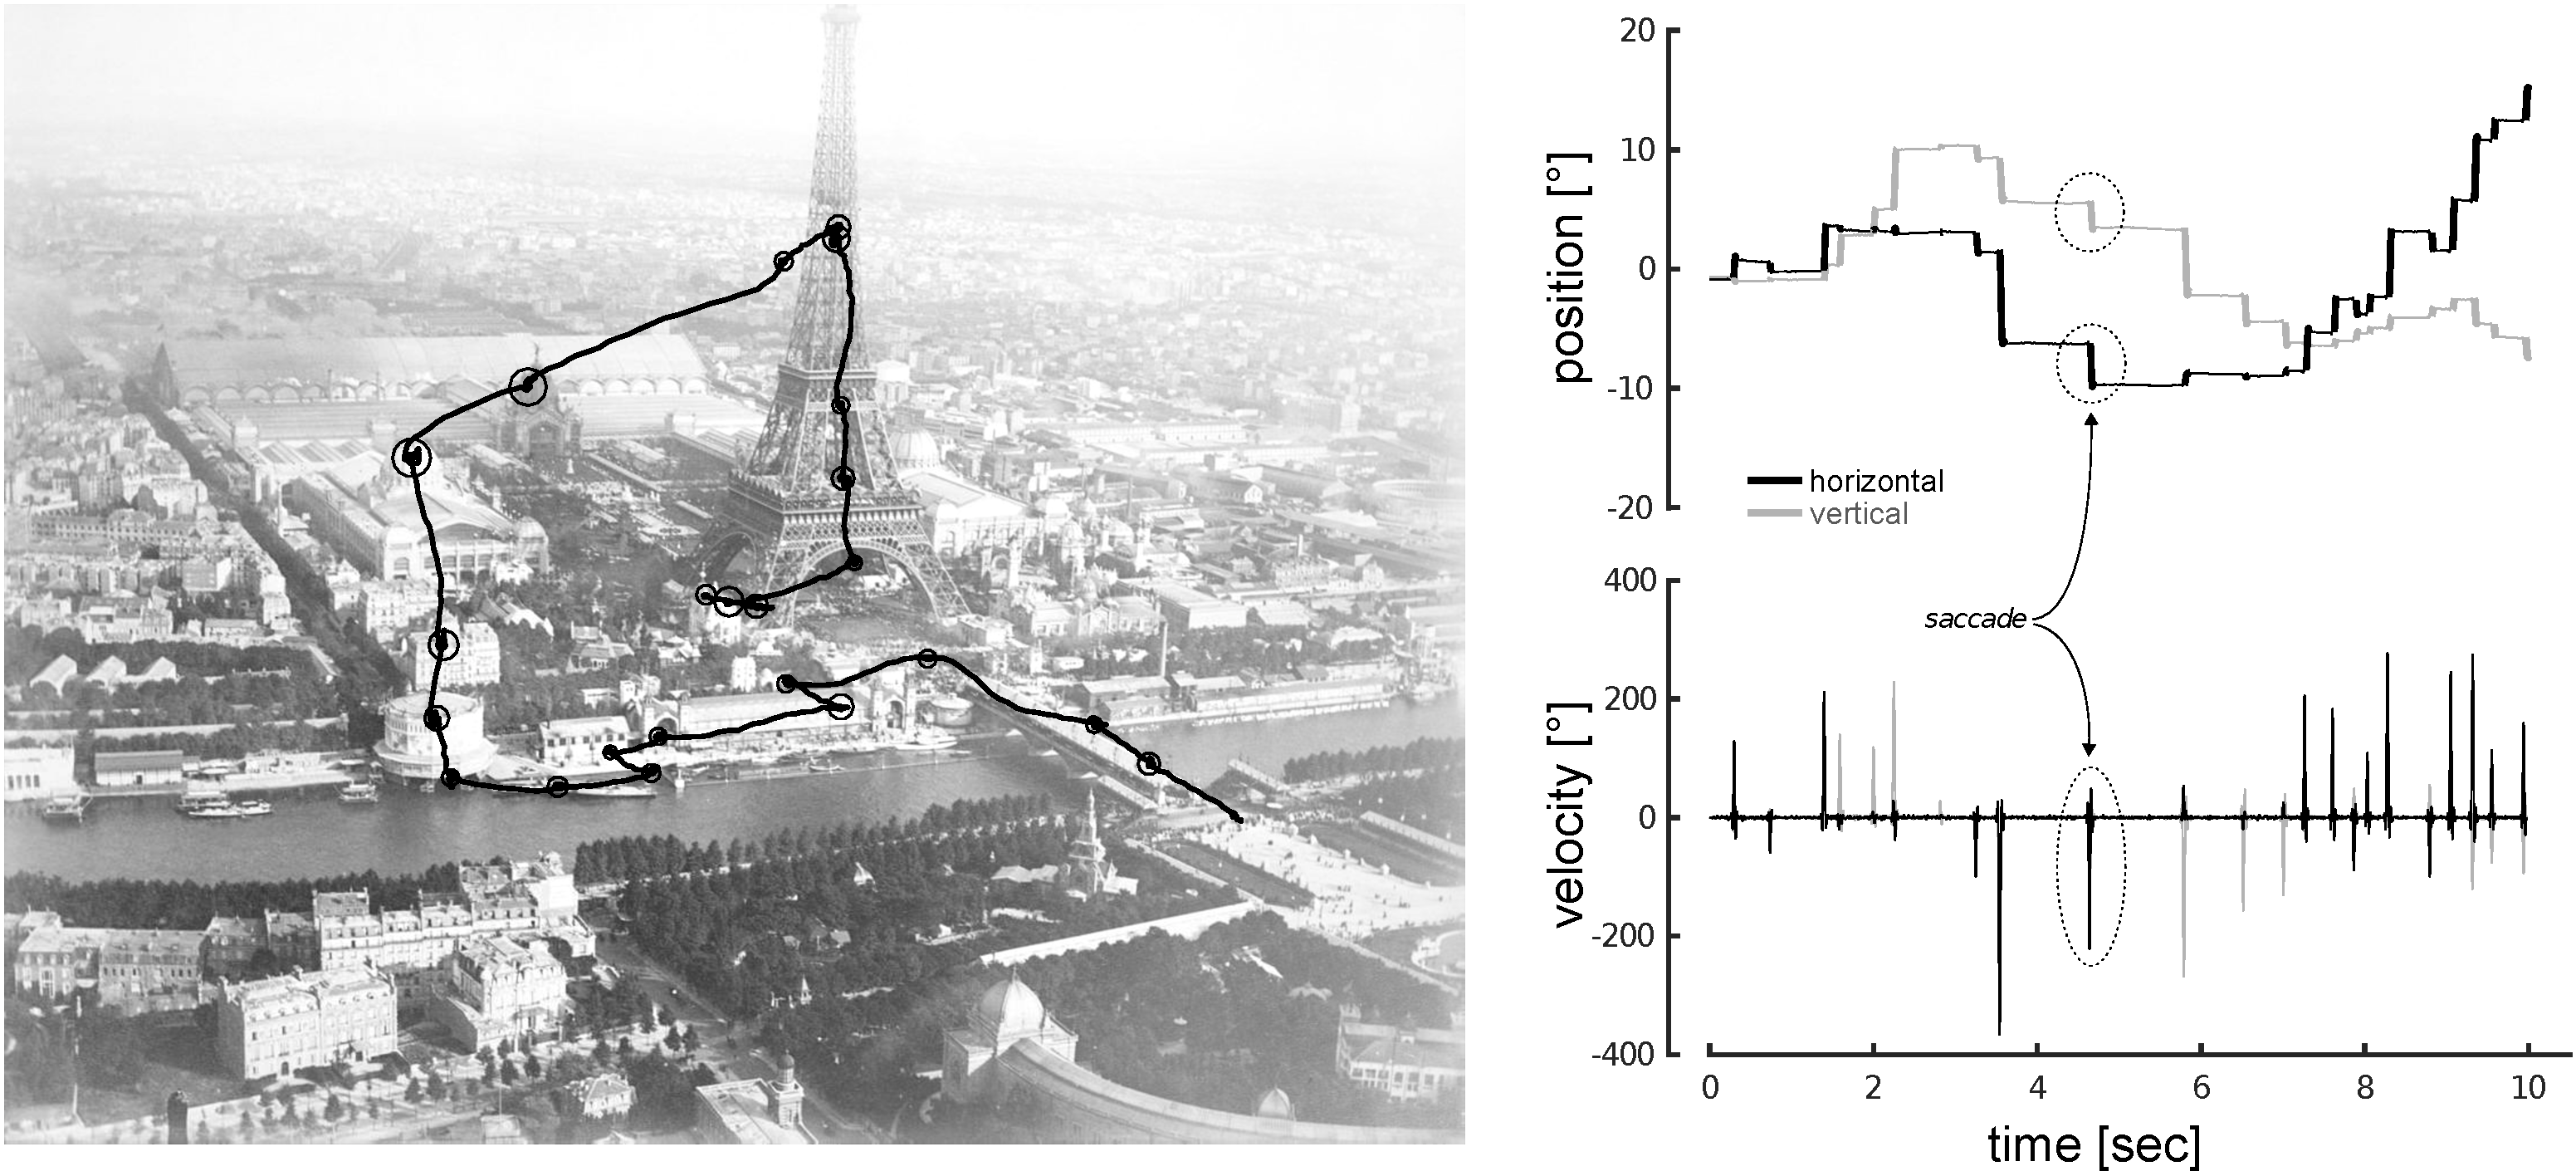
\includegraphics[width=148mm]{fig3.pdf}
\caption{Esempio di esplorazione visiva di una fotografia. L'immagine a sinistra mostra il percorso compiuto dallo sguardo (linea nera in sovraimpressione) di un soggetto durante 10 secondi di osservazione libera di una celebre fotografia di Alphonse Lièbert (1827-1913), rappresentante una visione aerea di Parigi durante l'Esposizione universale del 1889. Notare come l'esplorazione visiva segua gli elementi prominenti nell'immagine: inizia in posizione centrale seguendo la tour Eiffel, per poi dirigersi sui principali edifici circostanti. Nella figura i cerchi rappresentano la posizione dei periodi di fissazione (il diametro dei cerchi è una funzione della durata del periodo di fissazione). I due pannelli sulla destra della fotografia rappresentano il tracciato oculografico degli stessi 10 secondi di esplorazione visiva: il pannello in alto rappresenta la posizione (calcolata in gradi di angolo visivo rispetto al centro della fotografia) e il pannello in basso la velocità. Il tracciato oculografico illustra bene come l'esplorazione visiva sia costituita da una serie di momenti in cui gli occhi sono stazionari (fissazioni) e rapidi movimenti saccadici. Analizzare la velocità di spostamento dello sguardo permette facilmente di individuare le saccadi (che corrispondono ai picchi di velocità) e di conseguenza di isolare una fissazione dalla successiva. Notare come il profilo di accelerazione e decelerazione, ben visibile in Figura~\ref{fig2}, qui appaia quasi come un singolo impulso a causa della diversa scala temporale.}
\label{fig3}
\end{figure}

\break
\section{Movimenti oculari e processi cognitivi}

\subsection{Attenzione}
Il comportamento di esplorazione visiva è composto da una successione di fissazioni, intervallate da movimenti saccadici che orientano la fovea verso parti diverse dell'immagine (un esempio è rappresentato in figura~\ref{fig3}). La sequenza di saccadi e fissazioni eseguita durante l'osservazione di una scena visiva non è casuale ma è influenzata da stati mentali e obiettivi cognitivi dell'osservatore. Uno dei primi a mostrarlo è stato Alfred L. Yarbus (1914-1986), uno psicologo russo considerato come uno dei pionieri nello studio dei movimenti oculari. Tra gli anni '50 e '60 Yarbus utilizzò un innovativo metodo per la registrazione dei movimenti oculari, basato su minuscole ventose fissate sulla superficie dell'occhio, che gli permise di studiare i movimenti oculari con grande precisione. Yarbus osservò che i movimenti dello sguardo non sono casuali ma sono funzionali agli obiettivi percettivi e cognitivi dell'osservatore: durante l'osservazione di una scena lo sguardo si sofferma (sia volontariamente che involontariamente) più spesso e più a lungo  sugli elementi che sono suscettibili di apportare una maggiore quantità di informazioni. Vi è quindi un meccanismo in grado di filtrare l'informazione proveniente dalle parti periferiche del campo visivo e di selezionare gli elementi più salienti o rilevanti come potenziali bersagli dei prossimi movimenti saccadici. Questo meccanismo è l'attenzione visuo-spaziale: guardiamo ciò che attrae la nostra attenzione. 

Numerosi studi hanno dimostrato che esiste uno stretto rapporto tra la preparazione di un movimento oculare saccadico e l'orientamento \textit{implicito} (cioè in assenza di uno spostamento dell'asse visivo) dell'attenzione spaziale. Ad esempio si è osservato che l'esecuzione di un movimento saccadico è necessariamente preceduta dall'orientamento dell'attenzione implicita verso il bersaglio \cite{Deubel1996}. Questo orientamento dell'attenzione causa un miglioramento nella percezione dei dettagli visivi del bersaglio nell'intervallo immediatamente precedente all'esecuzione del movimento, cioè prima dello spostamento dell'asse visivo, quando la fovea è ancora orientata verso il punto di fissazione iniziale. È stato dimostrato anche il fenomeno complementare: orientare l'attenzione in una posizione dello spazio facilita la successiva esecuzione di un movimento saccadico verso quella stessa posizione spaziale \cite{Kowler1995}, riducendone la latenza (definibile come il tempo di reazione saccadico, cioè l'intervallo che intercorre tra l'apparizione di un bersaglio e l'esecuzione di una saccade verso di esso). 

Verso la fine degli anni ottanta, Rizzolatti e colleghi furono i primi a proporre che l'attenzione visuo-spaziale derivi proprio dall'attivazione degli stessi circuiti neurali implicati nella programmazione ed esecuzione dei movimenti saccadici \cite{Rizzolatti1987}, formulando la teoria \textit{premotoria} dell'attenzione. Secondo questa teoria orientare in maniera implicita l'attenzione verso una posizione spaziale è equivalente a programmare un movimento oculare verso quella posizione, senza però eseguirlo. Questa teoria è stata inizialmente proposta sulla base di esperimenti comportamentali, ma ha in seguito ricevuto un forte supporto anche da studi di neuroimaging \cite{Corbetta1998} e neurofisiologia \cite{Moore2001}. 

È interessante notare come uno degli studi che ha fornito l'impeto iniziale alla teoria premotoria sia stato basato sull'analisi delle traiettorie dei movimenti oculari saccadici. In questo studio \cite{Sheliga1995}, si misurarono le traiettorie, in particolare la curvatura, di saccadi verticali eseguite mentre l'attenzione era orientata nell'emispazio visivo destro o sinistro. L'intuizione alla base di questo studio è che se l'orientamento dell'attenzione implica un'attivazione dei circuiti oculomotori, questa attivazione dovrebbe manifestarsi come una modulazione del movimento saccadico. I risultati mostrarono che quando l'attenzione é orientata verso un emicampo visivo (destro o sinistro), la traiettoria del movimento saccadico verticale non é rettilinea ma presenta una sistematica deviazione, una curvatura in direzione dell'emicampo opposto (rispetto al focus dell'attenzione). I meccanismi attraverso cui si realizza questa modulazione della traiettoria dei movimenti saccadici sono ancora dibattuti \cite{VanderStigchel2006}, ma è evidente che questo risultato implica un certo grado di sovrapposizione tra i circuiti neurali che sottendono attenzione e movimenti saccadici, in accordo con la teoria premotoria e in contrasto con i modelli dell'attenzione precedenti, nei quali l'attenzione era vista piuttosto come un meccanismo di controllo sopra-modale anatomicamente separato dai circuiti motori. Questo studio rappresenta quindi un ottimo esempio di come l'analisi di alcuni parametri dei movimenti oculari possa fornire importanti elementi per la comprensione di processi più tipicamente cognitivi come l'attenzione.

\subsection{Cognizione numerica}
Nella sezione precedente è stato brevemente illustrato lo stretto legame tra movimenti oculari saccadici e attenzione visuo-spaziale. L'orientamento dell'attenzione nello spazio tuttavia non è implicato unicamente nella guida dei movimenti oculari o nella percezione visiva. Vi sono infatti altre operazioni cognitive, come la stima numerica, o la capacità di giudicare il più grande tra due numeri, che si pensa richiedano processi molto simili all'orientamento dell'attenzione nello spazio. Questa ipotesi è supportata da un grande numero di studi comportamentali e di neuroimmagine, che hanno dimostrato, ad esempio, come le aree celebrali della corteccia parietale posteriore che sono implicate nella programmazione di movimenti oculari svolgano un ruolo anche nell'esecuzione a mente di semplici operazioni aritmetiche come sottrazione o addizione \cite{Knops2009}. Questi studi suggeriscono che la rappresentazione mentale abbia una natura spaziale e che l'elaborazione di una grandezza numerica coinvolga l'orientamento dell'attenzione spaziale \cite{Hubbard2005}. 

Diversi ricercatori nel campo della cognizione numerica hanno quindi pensato di utilizzare l'analisi dei movimenti oculari per comprendere meglio la natura della rappresentazione mentale dei numeri. Loetscher e colleghi \cite{Loetscher2008} hanno registrato i movimenti oculari di soggetti impegnati in compiti di bisezione numerica, consistente nell'indicare il numero che si trova nel mezzo di una coppia di numeri (ad esempio il numero in mezzo per la coppia 1-9 è 5). Durante l'esecuzione del compito i soggetti erano in completa oscurità, in modo da non avere informazione visiva in ingresso che potesse guidare, ad esempio in maniera automatica o esogena, i movimenti oculari; i due numeri erano presentati acusticamente. I risultati mostrarono che la posizione orizzontale dello sguardo si spostava verso sinistra quando i due numeri erano presentati in ordine decrescente (9,1), ma non quando questi erano presentati in ordine crescente (1,9). Se consideriamo gli spostamenti degli occhi effettuati durante il compito come la manifestazione di spostamenti dell'attenzione nello spazio numerico mentale, questi supportano l'ipotesi che lo spazio numerico mentale sia organizzato come una linea numerica mentale, nella quale i numeri più piccoli sono rappresentati a sinistra \cite{Zorzi2002}. In uno studio successivo \cite{Loetscher2010}, si chiese ai soggetti di produrre una serie casuale di numeri, e si trovò che l'analisi dei movimenti oculari (gli spostamenti dell'asse visivo durante la produzione della sequenza numerica) permetteva di predire se il prossimo numero della serie sarebbe stato più grande o più piccolo del precedente, ancora prima che il soggetto lo pronunciasse. Questi risultati mostrano quindi come l'elaborazione di grandezze numeriche possa modulare il sistema oculomotorio; altri studi più recenti hanno adottato l'approccio opposto, e mostrato come l'esecuzione di movimenti oculari, sia automatici che volontari, possa influenzare l'elaborazione concomitante di grandezze numeriche \cite{Ranzini2015,Ranzini2016}. Ad esempio Ranzini e colleghi \cite{Ranzini2016} hanno osservato che in un compito di giudizio di parità numerica (nel quale i soggetti devono indicare il più velocemente possibile se un numero è pari o dispari) il tipico \textit{effetto grandezza}, caratterizzato da un rallentamento dei tempi di reazione con l'aumentare della grandezza numerica, scompare quando i soggetti effettuano simultaneamente dei movimenti oculari, sia saccadici che di inseguimento lento, verso il lato destro del campo visivo. Questo risultato avvalora l'ipotesi di una corrispondenza tra lo spazio visivo e lo spazio numerico mentale.

In conclusione questi studi, al di là della loro rilevanza per i modelli teorici della cognizione numerica, mostrano come l'analisi dei movimenti oculari possa essere utile anche nell'investigazione di processi cognitivi apparentemente più astratti, come quelli alla base della nostra abilità di eseguire operazioni numeriche.

\subsection{Pupillometria}

Nelle sezioni precedenti abbiamo discusso dei movimenti di rotazione dell'occhio nell'orbita. Vi è un'altra classe di movimenti oculari, alla quale non abbiamo ancora accennato, ma che ha notevolissime potenzialità di impiego nello studio dei processi cognitivi. Si tratta dei movimenti di dilatazione (detto anche \textit{midriasi}) e restringimento (o \textit{miosi}) della pupilla, cioè il foro situato al centro dell'iride che permette alla luce di entrare all'interno del bulbo oculare e raggiungere la retina. Il diametro della pupilla è determinato dalla contrazione di due muscoli opposti: lo \textit{sphincter pupillae} e \textit{dilator pupillae}. L'attivazione di questi muscoli è determinata principalmente dal livello di luce ambientale. Le variazioni nel diametro pupillare causate da variazioni nel livello di illuminazione sono infatti molto grandi, e facilmente visibili a occhio nudo: passare da una molto stanza illuminata ad una molto scura può causare una dilatazione del diametro pupillare fino al doppio della sua grandezza tipica, che si aggira intorno ai 3 millimetri \cite{MacLachlan2002}. Inoltre, poiché le fibre nervose che mediano dilatazione e restringimento della pupilla appartengono rispettivamente al sistema nervoso autonomo simpatico e parasimpatico, il diametro pupillare riflette anche stati psico-fisiologici come il livello di arousal. Infine, altre variazioni del diametro pupillare avvengono durante l'accomodazione.

Sovrapposte alle fluttuazioni del diametro pupillare dovute ad arousal, accomodazione e riflesso alla luce, vi sono altre variazioni caratterizzate da un'ampiezza molto minore (nell'ordine di 0,5 millimetri), che sono collegate all'attività cognitiva. Poiché queste variazioni hanno un'ampiezza molto bassa, e tendono ad essere mascherate da quelle più ampie indotte da cambiamenti nel livello di illuminazione o arousal, è necessario estrarle con un procedimento molto simile a quello utilizzato nell'analisi dei potenziali evocati elettroencefalografici. In breve, il diametro pupillare viene registrato per numerose ripetizioni dello stimolo o del compito di interesse; durante l'analisi, le diverse "epoche" di registrazione vengono sincronizzate con gli eventi stimolanti, per poi essere mediate (averaging), in modo da isolare la risposta pupillare causata dall'evento di interesse dal rumore di fondo e dalle variazioni dovute ad altri fattori (ad esempio l'arousal, o viceversa la stanchezza del soggetto). 

Moltissimi studi hanno utilizzato questa tecnica (per una rassegna si veda \cite{Beatty2000}) e mostrato che una dilatazione del diametro pupillare accompagna ogni sforzo, sia che si tratti di uno sforzo fisico (ad esempio sollevare un peso) sia di uno sforzo puramente mentale, come risolvere un problema aritmetico \cite{Hess1964} o mantenere in memoria una sequenza di numeri \cite{Kahneman1966}. I meccanismi attraverso i quali l'attività cognitiva si riflette nella dilatazione del diametro pupillare sono ancora oggetto di indagine, ma in generale è ritenuto che si tratti di una conseguenza dell'attivazione dei neuroni noradrenergici nel locus coeruleus (una struttura del tronco encefalico) e del conseguente rilascio di noradrenalina \cite{Aston-Jones2005}. In particolare la dilatazione della pupilla sarebbe correlata con un'attivazione del sistema noradrenergico, il quale ha un ruolo importante non solo nella regolazione dell'arousal e nel mantenimento dello stato di veglia, ma anche in molte altre funzioni cognitive. Ad esempio, è ritenuto svolgere un ruolo nel controllo dell'attenzione e nella sua focalizzazione \cite{Corbetta2008}: quando l'attenzione è focalizzata su un compito il sistema noradrenergico presenterebbe un modo di funzionamento fasico, caratterizzato cioè da periodi di bassa attività spontanea interrotti da rapide attivazioni associate ai processi decisionali relativi al compito. Queste oscillazioni fasiche si rifletterebbero nel diametro pupillare e la loro ampiezza sarebbe correlata con il carico attentivo richiesto. In accordo con questa ipotesi è stato dimostrato che, in un compito di identificazione di brevi stimoli visivi e uditivi, l'ampiezza della dilatazione pupillare evocata è correlata con la difficoltà del compito e con il carico attentivo richiesto per svolgerlo \cite{Lisi2015b}. 

Per concludere, è opportuno sottolineare che il diametro pupillare, grazie alla sua relazione con il sistema noradrenergico, può essere utile nello studio di molti processi cognitivi implicati nella presa di decisione \cite{Nieuwenhuis2005}, non solamente l'attenzione. È prevedibile che la misurazione del diametro pupillare assumerà un ruolo sempre più importante nei prossimi anni, grazie anche al fatto che può essere effettuata molto facilmente e in maniera non-invasiva.

\section{Tecniche di registrazione dei movimenti oculari}
Le prime tecniche utilizzate per analizzare o registrare i movimenti oculari erano spesso invasive (si pensi ad esempio alle minuscole ventose applicate sugli occhi da Yarbus negli anni '60). Altri metodi meno invasivi erano anche meno accurati, come l'elettrooculografia (EOG), ad esempio, che si basa sul potenziale corneo-retinico, cioè la differenza di potenziale elettrico, dell'ordine di circa 1 mV, esistente tra la cornea e il \textit{fundus} dell'occhio (la faccia interiore dell'occhio, opposta al cristallino, dove è situata la retina). Per via di questo potenziale l'occhio può essere considerato come un dipolo elettrico (con polo negativo sulla retina), le cui rotazioni danno origine a segnali che possono essere misurati tramite elettrodi posti in prossimità degli occhi. Tuttavia, il potenziale corneo-retinico non è costante ed è influenzato da numerosi fattori (ad esempio illuminazione ed affaticamento) attraverso meccanismi ancora non completamente chiariti; di conseguenza la precisione di questa tecnica è molto limitata. 

Un metodo molto più accurato per registrare i movimenti oculari è quello della bobina sclerale (\textit{scleral coil}) che però richiede l'applicazione di una speciale lente a contatto, al cui interno è presente la bobina. La testa del soggetto in questo caso deve essere posizionata dentro un campo magnetico: quando la bobina è immersa nel campo magnetico, genera un potenziale elettrico che è in funzione dell'angolo tra orientamento della bobina e direzione del campo magnetico. Questo metodo offre la migliore accuratezza (nell'ordine di 0.01$^{\circ}$), ma a causa della sua invasività (la lente a contatto risulta particolarmente scomoda data la presenza della bobina e di un filo elettrico che fuoriesce dalla lente) non è utilizzato molto frequentemente.

Al giorno d'oggi, sono invece disponibili molti sistemi di oculometria detti video-oculografici (\textit{video-based eyetrackers}) che, pur non essendo invasivi, permettono di raggiungere eccellenti livelli di accuratezza, tali da permettere anche di analizzare i microscopici movimenti oculari effettuati durante i periodi di fissazione. Questi sistemi si basano sull'analisi dell'immagine dell'occhio ripresa da una telecamera. Allo scopo di misurare la direzione dello sguardo in maniera accurata, la telecamera è affiancata da una sorgente luminosa (tipicamente caratterizzata da una frequenza inferiore a quella della luce visibile, cioè nella regione dell'infrarosso). La luce proveniente da questa sorgente luminosa colpisce l'occhio generando un'immagine riflessa, detta anche immagine primaria di Purkinje (causata dalla luce riflessa sulla superficie esterna della cornea). Per distinguere i movimenti della testa dai movimenti dell'occhio, le immagini in arrivo dalla telecamera sono processate in tempo reale così da identificare sia il riflesso di Purkinje che la pupilla (in particolare il centro della pupilla). La posizione del centro della pupilla rispetto al riflesso di Purkinje cambia con le rotazioni dell'occhio nell'orbita, ma rimane relativamente costante a seguito di piccoli movimenti della testa. Questo metodo permette quindi di isolare i movimenti degli occhi rispetto ai movimenti della testa, e di ottenere un accurato monitoraggio della direzione dello sguardo anche in casi in cui la testa non sia perfettamente immobilizzata. I modelli più recenti hanno frequenze di campionamento molto alte, fino anche a 2000~Hz, che permettono quindi di registrare i movimenti oculari con eccellente precisione temporale. La precisione spaziale di questi sistemi può anche essere ulteriormente aumentata se si includono le immagini secondarie di Purkinje, dovute ai riflessi che si creano sulla superficie interna della cornea, e sulle superfici interna ed esterna del cristallino.  

\section{Sommario}
In questo capitolo abbiamo descritto i principali tipi di movimenti oculari, e le loro caratteristiche funzionali e fisiologiche. Lo studio dei movimenti oculari riveste innanzitutto un ruolo fondamentale nello studio della percezione visiva: abbiamo infatti descritto la visione come un processo attivo, nel quale l'esperienza visiva del mondo circostante dipende dall'integrazione dell'informazione visiva proiettata sulla retina con segnali extra-retinici collegati alle rotazioni dell'occhio nell'orbita. Inoltre abbiamo visto come la programmazione dei movimenti oculari sia strettamente legata all'orientamento dell'attenzione visuo-spaziale, e come questo legame permetta di utilizzarli nello studio di processi cognitivi apparentemente più astratti ma basati su rappresentazioni mentali organizzate in maniera spaziale, come l'elaborazione di quantità numeriche. Infine, abbiamo trattato brevemente i movimenti di dilatazione e restringimento della pupilla, e visto come possano fornire informazioni riguardo l'attività del sistema noradrenergico, e quindi su tutti i processi cognitivi collegati al neurotrasmettitore noradrenalina. 

In conclusione, abbiamo mostrato come l'analisi dei movimenti oculari possa fornire una preziose informazioni riguardo i processi cognitivi e gli stati mentali di un soggetto, ed è quindi particolarmente promettente nell'ambito della neuropsicologia cognitiva, in quanto può essere abbinata alla maggior parte dei protocolli sperimentali attualmente utilizzati con costi relativamente limitati.


\bibliographystyle{abbrv}
\bibliography{\myreferences} % note that this is called using the command defined at the beginning

\end{document}
